\chapter{Implementacija i korisničko sučelje}
		
		
		\section{Korištene tehnologije i alati}

             \subsection{Korišteni alati}
                \par    Alati koji su bili korišteni za izradu aplikacije nisu divergirali od standarda u industriji. Za pisanje
                programskog koda i skripti, sa poslužiteljske i korisničke strane, korišten je Microsoftov Visual Studio Code. 
                Jednostavan program čija osnovna funkcionalnost uključuje sve klasične operacije nad tekstom koji predstavlja kod:
                automatsko naglašavanje teksta bojom ovisno o programskom jeziku koji se koristi, mnoštvo kratica 
                na tipkovnici za manipulaciju teksta, ubacivanje ili uklanjanje komentara, tabulatora i sl. VSC se također može 
                specijalizirati za razvoj bilo koje vrste projekta pomoću dodataka koji su javno dostupni svima i mogu se 
                opcionalno instalirati.
                
                \par Za bazu podataka je korišten pgAdmin. Program unutar kojeg se koristi SQL kako bi se definirala relacijska baza
                podataka, sve njene tablice, te konačno, podatci. Poveznicu između njih čini kod napisan za poslužiteljsku stranu 
                u Pythonu, čije su krajnje API točke testirane pomoću alata Postman. Postman omogućuje slanje HTTP zahtjeva na 
                bilo koju adresu, te dopušta apsolutnu kontrolu nad poslanim paketom. Pomoću tog alata je testirano prima
                li poslužiteljska strana pravilno informacije koje se pošalju (npr. informacije za registraciju), ili dobivaju li
                se točni podatci iz baze kad ih se zatraži (npr. sve riječi nekog rječnika).

            \subsection{Korištene tehnologije}
                    Korištene tehnologije su sve u skladu razvoja RESTful aplikacije, što samo zapravo znači da se komunikacija
                klijenta i poslužitelja odvija preko HTTP ili HTTPS protokola, sa GET, POST, PUT i DELETE zahtjevima. 
                
                \par    Na korisničkoj strani je korišten javascript radni okvir React, koji je razvila Meta (bivši Facebook), koji je 
                zasnovan na komponentama. Svaka komponenta može imati svoju definiranu funkcionalnost, te može sadržavati druge predefinirane, 
                ili korisnički definirane komponente.

                \par    Za neke dijelove korisničkog sučelja je korišten MUI (Material User Interface) koji ima nekolicinu predefiniranih
                komponenti, kao npr. gumbe, tablice ili kartice za prikaz podataka. MUI je napravljen za React i ne može se koristiti
                sa nekom drugom bibliotekom.

                \par    Za pamćenje stanja aplikacije (tzv. State) je korišten Redux. Redux je mala biblioteka sa jednostavnim API-em.
                Bazirana je na logici da svako novo stanje aplikacije je redukcija prijašnjeg, što zapravo znači da se
                svako novo stanje računa pomoću reducijske funkcije. Kao prvi argument uzima trenutno stanje, a kao drugi
                argument akciju pomoću koje izmjeni trenutno stanje kako bi dobili sljedeće. Ukupno stanje aplikacije se 
                dijeli u tzv. kriške (slices), od kojih je svaka odgovorna za praćenje stanja jednog dijela aplikacije (npr.
                trenutno odabrani jezik ili trenutno stanje odabranog rječnika).

                \par    Za dohvaćanje podataka je korišten Axios, biblioteka utemeljena na obećanjima (u javascriptu) koja služi
                za slanje zahtjeva bilo kojem poslužitelju. 

                \par    Na poslužiteljskoj strani je implementacijski jezik Python, a korištene biblioteke su Flask i nekolicina popratnih
                tehnologija koje služe za proširivanje funkcionalnosti Flaska, kao što su Marshmellow i SQL-Alchemy, čiji su
                zadatci ORM (Object Relational Mapping). Marshmellow je agnostičan na radne okvire, tj može se koristiti sa bilo
                kojim radnim okvirom u pythonu, dok za korištenje SQL-Alchemy je korišten nastavak Flask-SQLAlchemy. 

            \subsection{Poveznice na korištene tehnologije i alate}
            \begin{itemize}
                \item \href{https://code.visualstudio.com/}{Visual Studio Code}
                \item \href{https://www.pgadmin.org/}{PgAdmin}
                \item \href{https://www.postman.com/}{PostMan}
                \item \href{https://www.python.org/}{Python}
                \item \href{https://flask.palletsprojects.com/en/3.0.x/}{Biblioteka Flask}
                \item \href{https://marshmallow.readthedocs.io/en/stable/}{Biblioteka Marshmellow}
                \item \href{https://flask-sqlalchemy.palletsprojects.com/en/3.1.x/}{Biblioteka Flask-SQLAlchemy}
                \item \href{https://react.dev/}{Biblioteka React}
                \item \href{https://mui.com/}{Biblioteka MUI}
                \item \href{https://redux.js.org/}{Redux}
                \item \href{https://axios-http.com/docs/intro}{Axios}
              \end{itemize}
			\eject 
		
	
		\section{Ispitivanje programskog rješenja}
			
			\textbf{\textit{dio 2. revizije}}\\
			
			 \textit{U ovom poglavlju je potrebno opisati provedbu ispitivanja implementiranih funkcionalnosti na razini komponenti i na razini cijelog sustava s prikazom odabranih ispitnih slučajeva. Studenti trebaju ispitati temeljnu funkcionalnost i rubne uvjete.}
	
			
			\subsection{Ispitivanje komponenti}
			\textit{Potrebno je provesti ispitivanje jedinica (engl. unit testing) nad razredima koji implementiraju temeljne funkcionalnosti. Razraditi \textbf{minimalno 6 ispitnih slučajeva} u kojima će se ispitati redovni slučajevi, rubni uvjeti te izazivanje pogreške (engl. exception throwing). Poželjno je stvoriti i ispitni slučaj koji koristi funkcionalnosti koje nisu implementirane. Potrebno je priložiti izvorni kôd svih ispitnih slučajeva te prikaz rezultata izvođenja ispita u razvojnom okruženju (prolaz/pad ispita). }
			
			 

			\subsection{Ispitivanje sustava}
Ispitivanje sustava ostvareno je Selenium WebDriverom u Pythonu. Selenium WebDriver je alat za automatizaciju web preglednika. WebDriver koristi preglednikove vlastite mehanizme za kontrolu, čime osigurava visoku razinu realističnosti u testiranju, što ga čini ključnim alatom u razvoju softvera i osiguravanju kvalitete web aplikacija. Provedeni testovi s kodom priloženi su u nastavku.
\break

\begin{figure}[htp]
    \caption{prvi ispitni slučaj koji obrađuje ispravnu prijavu. Očekivani izlaz je uspješna prijava i preusmjeravanje.}
    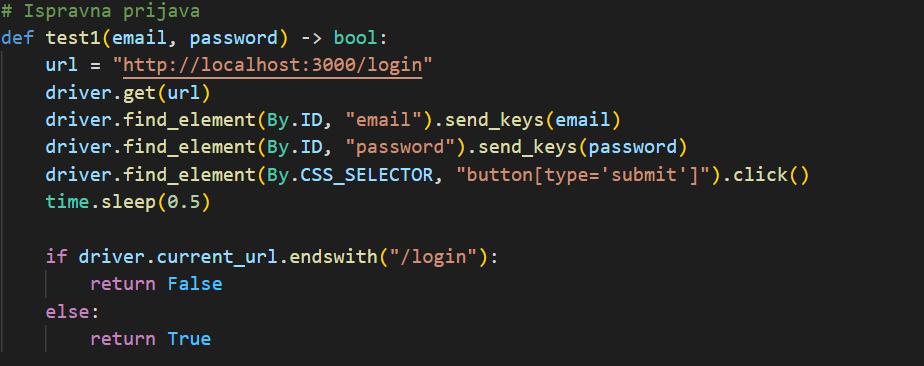
\includegraphics[scale=0.5]{dijagrami/test1.png}
    \centering
    
\end{figure}
\break

\begin{figure}[htp]
    \caption{drugi ispitni slučaj koji obrađuje neispravnu registraciju. Unosom maila u krivom formatu očekivani izlaz je neuspjela registracija.}
    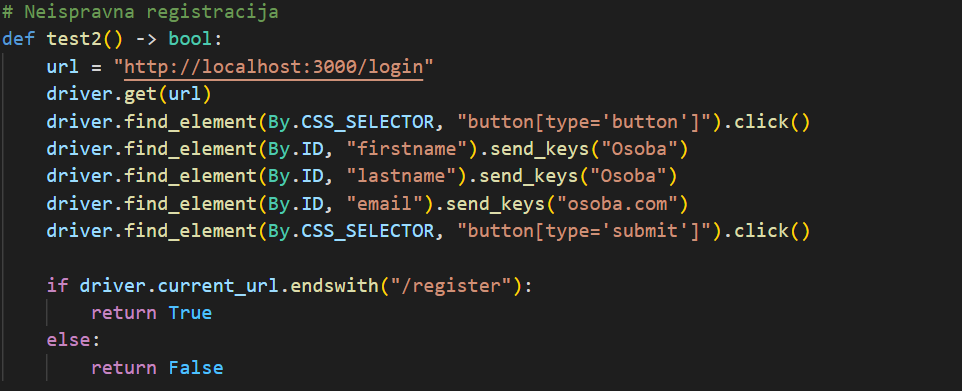
\includegraphics[scale=0.5]{dijagrami/test2.png}
    \centering
    
\end{figure}
\break

\begin{figure}[htp]
    \caption{treći ispitni slučaj koji obrađuje uspješnu promjenu lozinke. Preduvjet za promjenu lozinke je uspješna prijava u sustav kao student. Unosom podudarajućih lozinki očekivani izlaz je izmjena lozinke i preusmjeravanje.}
    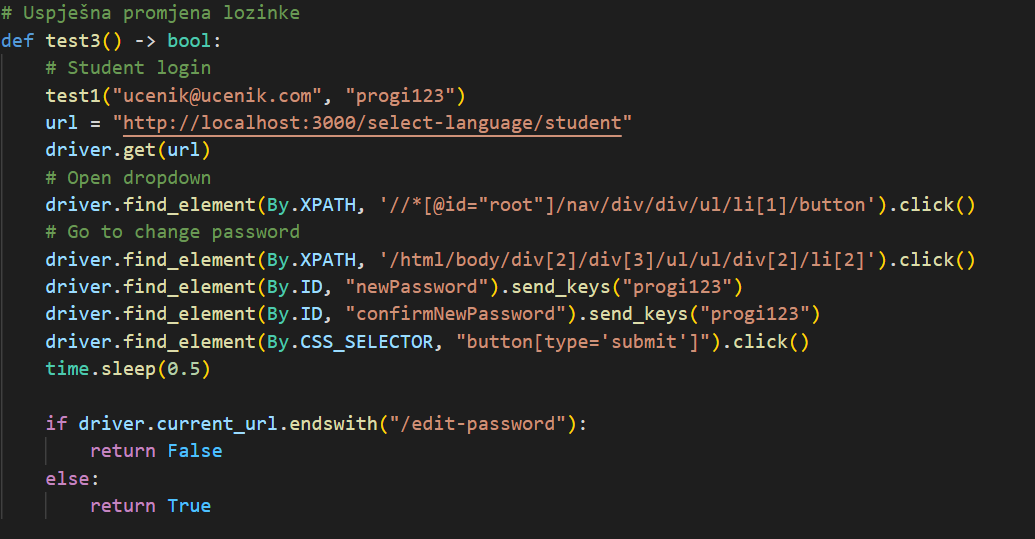
\includegraphics[scale=0.5]{dijagrami/test3.png}
    \centering
    
\end{figure}
\break

\begin{figure}[htp]
    \caption{četvrti ispitni slučaj koji obrađuje neispravno stvaranje admina. Preduvjet za stvaranje admina je uspješna prijava u sustav kao admin. Unosom nepodudarajućih lozinki u predložak, očekivani izlaz je neuspjela kreacija admina.}
    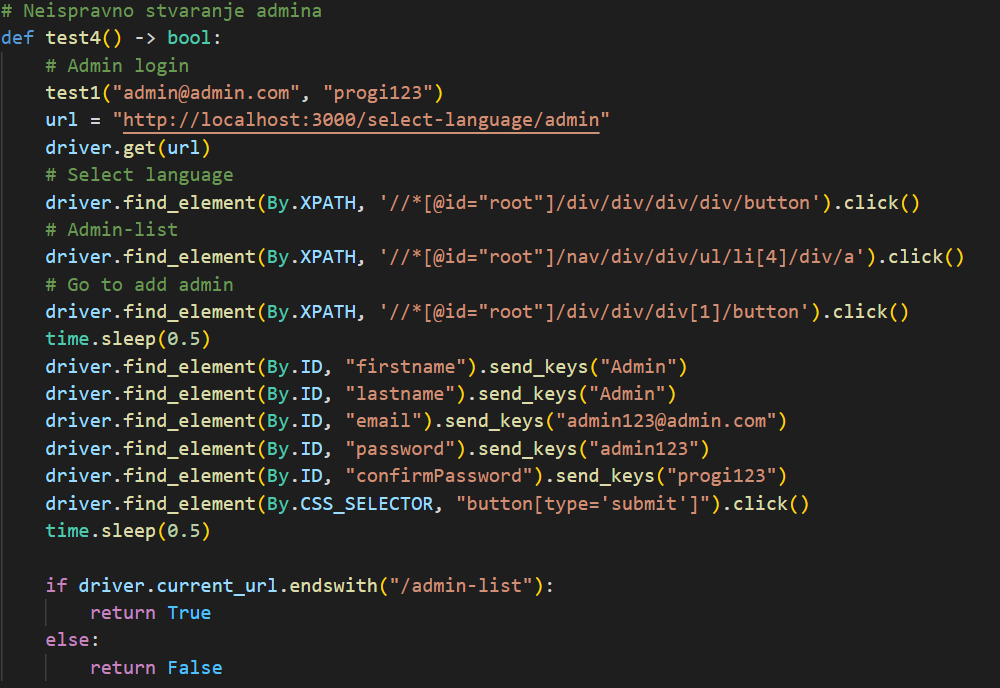
\includegraphics[scale=0.5]{dijagrami/test4.png}
    \centering
    
\end{figure}
\break

\begin{figure}[htp]
    \caption{peti ispitni slučaj koji obrađuje stvaranje rječnika s praznim imenom. Preduvjet za stvaranje rječnika je uspješna prijava u sustav kao admin. Bez unosa imena novog rječnika očekivani izlaz je nepromijenjeno stanje tablice rječnika u sustavu.}
    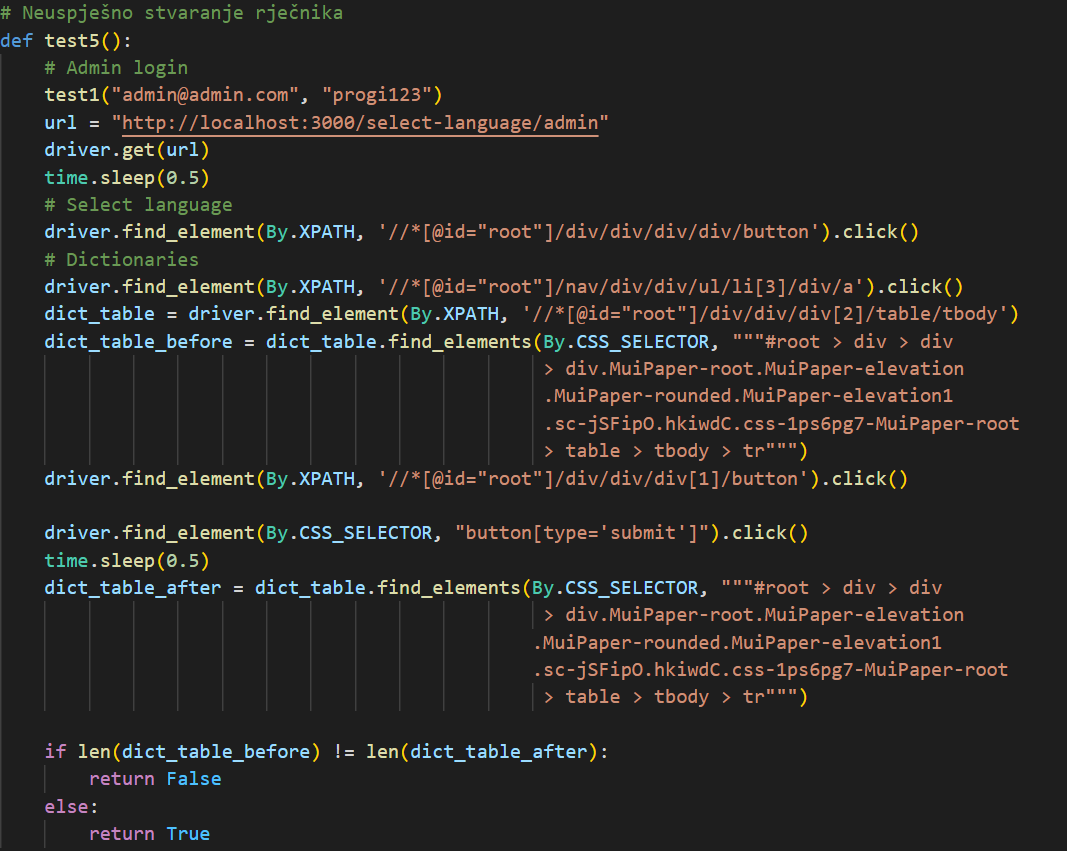
\includegraphics[scale=0.5]{dijagrami/test5.png}
    \centering
    
\end{figure}
\break

\begin{figure}[htp]
    \caption{terminal nakon pokretanja testova ispitivanja sustava.}
    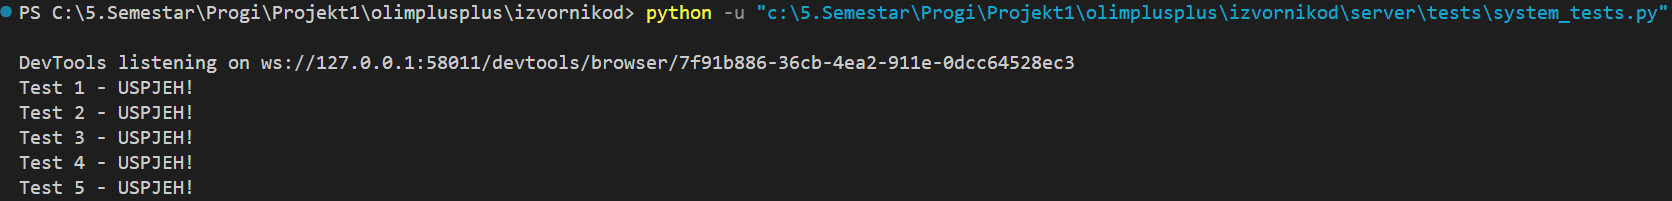
\includegraphics[scale=0.4]{dijagrami/terminal_screen.png}
    \centering
    
\end{figure}
\eject

		
		\section{Dijagram razmještaja}
			
		\begin{figure}[htp]
			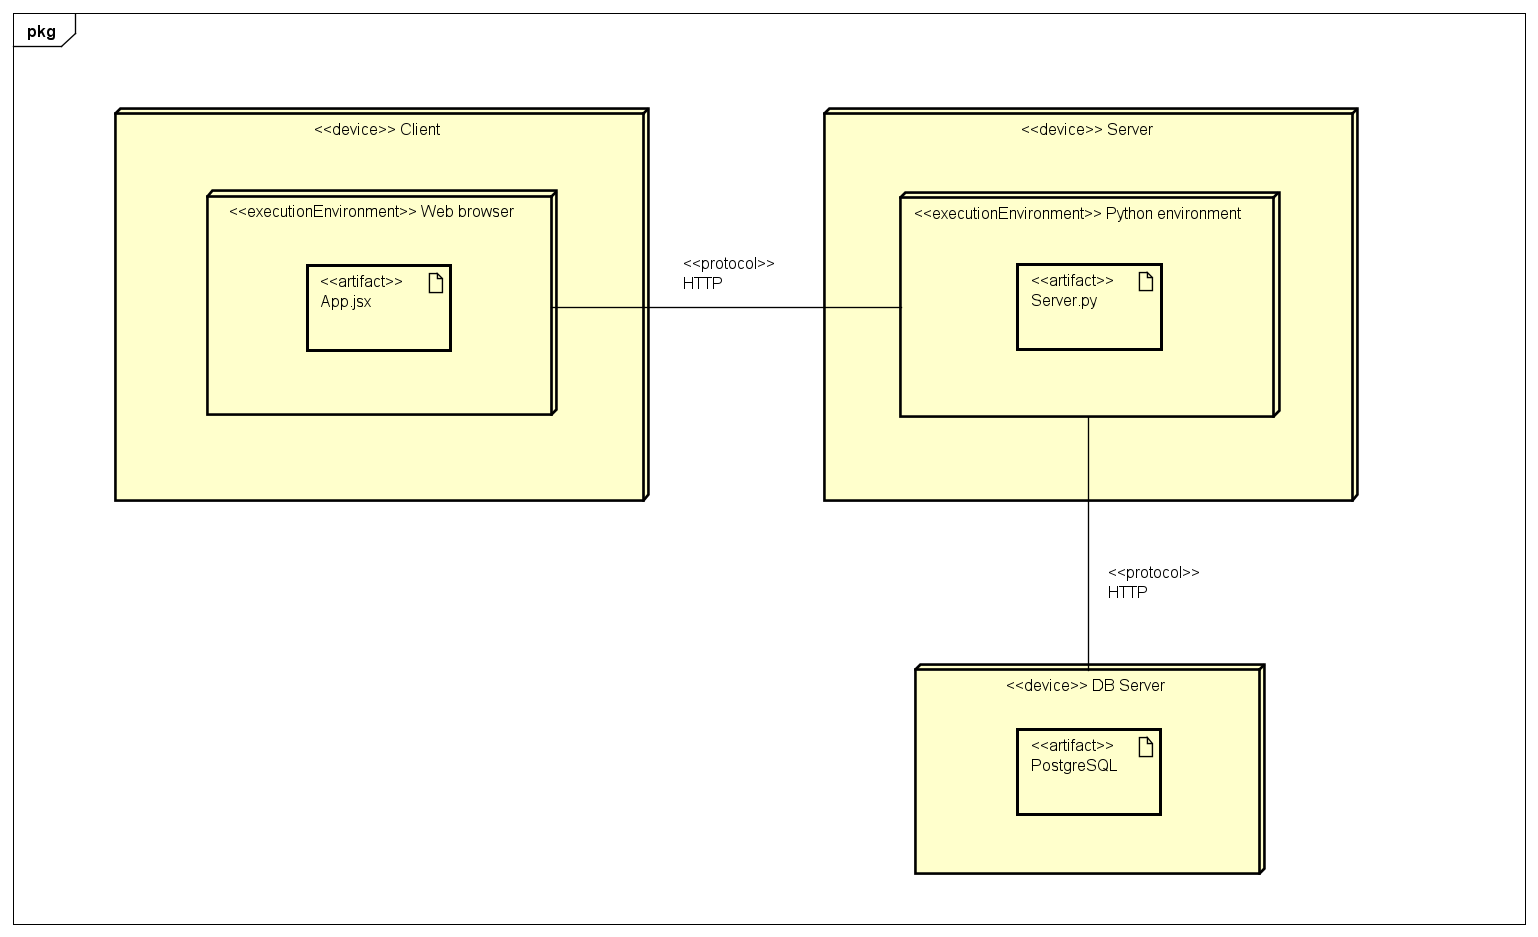
\includegraphics[scale=0.4]{dijagrami/DeploymentDiagram0.png}
			\centering
			\caption{Dijagram razmještaja}
		\end{figure}
		
		\section{Upute za puštanje u pogon}
		
			\textbf{\textit{dio 2. revizije}}\\
		
			 \textit{U ovom poglavlju potrebno je dati upute za puštanje u pogon (engl. deployment) ostvarene aplikacije. Na primjer, za web aplikacije, opisati postupak kojim se od izvornog kôda dolazi do potpuno postavljene baze podataka i poslužitelja koji odgovara na upite korisnika. Za mobilnu aplikaciju, postupak kojim se aplikacija izgradi, te postavi na neku od trgovina. Za stolnu (engl. desktop) aplikaciju, postupak kojim se aplikacija instalira na računalo. Ukoliko mobilne i stolne aplikacije komuniciraju s poslužiteljem i/ili bazom podataka, opisati i postupak njihovog postavljanja. Pri izradi uputa preporučuje se \textbf{naglasiti korake instalacije uporabom natuknica} te koristiti što je više moguće \textbf{slike ekrana} (engl. screenshots) kako bi upute bile jasne i jednostavne za slijediti.}
			
			
			 \textit{Dovršenu aplikaciju potrebno je pokrenuti na javno dostupnom poslužitelju. Studentima se preporuča korištenje neke od sljedećih besplatnih usluga: \href{https://aws.amazon.com/}{Amazon AWS}, \href{https://azure.microsoft.com/en-us/}{Microsoft Azure} ili \href{https://www.heroku.com/}{Heroku}. Mobilne aplikacije trebaju biti objavljene na F-Droid, Google Play ili Amazon App trgovini.}
			
			
			\eject 